\documentclass[10pt]{beamer}

% --- Modern Theme ---
\usetheme{metropolis}
\usecolortheme{default}
\setbeamercolor{background canvas}{bg=white}
\metroset{sectionpage=none,subsectionpage=none}

% --- Packages ---
\usepackage[utf8]{inputenc}
\usepackage{booktabs}
\usepackage{array}
\usepackage{tabularx}
\usepackage{amsmath}
\usepackage{amssymb}
\usepackage[scale=2]{ccicons}
\usepackage{pgfplots}
\usepgfplotslibrary{dateplot,fillbetween}
\usepackage{xspace}
\usepackage{tikz}
\usetikzlibrary{shapes.geometric, arrows.meta, positioning, fit, calc, decorations.pathreplacing, backgrounds}

% --- TikZ Styles ---
\tikzset{
  box/.style={rectangle, rounded corners=3pt, draw=mDarkTeal, fill=mDarkTeal!10,
              minimum width=2.2cm, minimum height=0.65cm, font=\small, align=center},
  bigbox/.style={rectangle, rounded corners=4pt, draw=mDarkTeal, fill=mDarkTeal!8,
              minimum width=3.2cm, minimum height=0.8cm, font=\small, align=center},
  arrow/.style={-Stealth, thick, draw=mDarkTeal},
  alertbox/.style={rectangle, rounded corners=3pt, draw=orange!80!black, fill=orange!10,
              minimum width=2.2cm, minimum height=0.65cm, font=\small, align=center},
  greenbox/.style={rectangle, rounded corners=3pt, draw=green!60!black, fill=green!10,
              minimum width=2.2cm, minimum height=0.65cm, font=\small, align=center},
  treeleaf/.style={rectangle, rounded corners=3pt, draw=green!60!black, fill=green!10,
              minimum width=1.5cm, minimum height=0.55cm, font=\scriptsize, align=center},
  treenode/.style={diamond, draw=mDarkTeal, fill=mDarkTeal!12,
              minimum width=1.7cm, minimum height=0.75cm, font=\scriptsize, align=center, aspect=2},
}

% --- Title Information ---
\title{Foundations of Artificial Intelligence}
\subtitle{Part IV: Machine Learning}
\institute{Department of Computer Science}
\date{}

\begin{document}

\maketitle

\begin{frame}{Lecture Roadmap}
    \setbeamertemplate{section in toc}[sections numbered]
    \tableofcontents[hideallsubsections]
\end{frame}

\begin{frame}{Learning Objectives}
    By the end of this lecture, you should be able to:
    \begin{itemize}
        \item Explain what \textbf{learning} means in the context of AI.
        \item Distinguish \textbf{supervised} from \textbf{unsupervised} learning.
        \item Understand the roles of \textbf{training} and \textbf{testing} data.
        \item Recognise and reason about \textbf{overfitting} and \textbf{underfitting}.
        \item Describe four fundamental algorithms: Linear Regression, k-NN, Decision Trees, k-Means.
    \end{itemize}
\end{frame}

% ======================================================
\section{What Is Learning?}
% ======================================================

\begin{frame}{What Does It Mean To Learn?}
    \textit{``A computer program is said to learn from experience $E$ with respect to tasks $T$ and performance measure $P$, if its performance on $T$ improves with $E$.''} \hfill — Tom Mitchell, 1997

    \vspace{0.4cm}
    \begin{center}
    \resizebox{0.82\textwidth}{!}{%
    \begin{tikzpicture}[node distance=0.95cm]
      \node[box] (E) {Experience\\(Data)};
      \node[bigbox, right=1.0cm of E] (L) {\textbf{Learning}\\Algorithm};
      \node[box, right=1.0cm of L] (M) {Model};
      \node[box, right=1.0cm of M] (P) {Better\\Performance};
      \draw[arrow] (E) -- (L);
      \draw[arrow] (L) -- (M);
      \draw[arrow] (M) -- (P);
    \end{tikzpicture}
    }
    \end{center}
    \vspace{0.25cm}
    Unlike classical AI (hand-coded rules), ML \textbf{discovers} patterns\\
    automatically from data.
\end{frame}

\begin{frame}{Classical AI vs Machine Learning}
    \begin{columns}[T,onlytextwidth]
        \column{0.48\textwidth}
        \alert{Classical / Rule-Based AI}
        \vspace{0.2cm}

        \begin{center}
        \begin{tikzpicture}[node distance=0.7cm]
          \node[box] (rules) {Rules (hand-crafted)};
          \node[box, below=of rules] (data) {New Data};
          \node[greenbox, below=0.5cm of data] (ans) {Answer};
          \draw[arrow] (rules) -- (data);
          \draw[arrow] (data) -- (ans);
        \end{tikzpicture}
        \end{center}

        \column{0.48\textwidth}
        \alert{Machine Learning}
        \vspace{0.2cm}

        \begin{center}
        \begin{tikzpicture}[node distance=0.7cm]
          \node[box] (data2) {Data + Answers};
          \node[box, below=of data2] (ml) {ML Algorithm};
          \node[greenbox, below=0.5cm of ml] (model) {Model (Rules)};
          \draw[arrow] (data2) -- (ml);
          \draw[arrow] (ml) -- (model);
        \end{tikzpicture}
        \end{center}
    \end{columns}
    \vspace{0.3cm}
    \textit{ML inverts the classical pipeline: we provide data and desired outputs; the algorithm finds the mapping.}
\end{frame}

\begin{frame}{Why Machine Learning Now?}
    \begin{enumerate}
        \item \textbf{Big Data:} billions of digital interactions every day.
        \item \textbf{Compute:} GPUs, cloud, specialised hardware.
        \item \textbf{Algorithms:} decades of research reaching maturity.
        \item \textbf{Open ecosystems:} Python, scikit-learn, PyTorch, etc.
    \end{enumerate}
    \vspace{0.3cm}
    Real applications: spam filtering, product recommendations, medical diagnosis, fraud detection, voice assistants.
\end{frame}

% ======================================================
\section{Supervised vs Unsupervised Learning}
% ======================================================

\begin{frame}{The Two Main Paradigms}
    \begin{center}
  \resizebox{0.76\textwidth}{!}{%
  \begin{tikzpicture}[node distance=1.0cm]
      \node[bigbox, fill=mDarkTeal!15] (ml) {\textbf{Machine Learning}};

      \node[bigbox, below left=0.9cm and 0.5cm of ml] (sup) {Supervised\\Learning};
      \node[bigbox, below right=0.9cm and 0.5cm of ml] (unsup) {Unsupervised\\Learning};

      \node[box, below=0.75cm of sup, xshift=-1.1cm] (cls) {Classification};
      \node[box, below=0.75cm of sup, xshift=1.1cm]  (reg) {Regression};

      \node[box, below=0.75cm of unsup, xshift=-1.1cm] (clu) {Clustering};
      \node[box, below=0.75cm of unsup, xshift=1.1cm]  (dim) {Dim.\ Reduction};

      \draw[arrow] (ml) -- (sup);
      \draw[arrow] (ml) -- (unsup);
      \draw[arrow] (sup) -- (cls);
      \draw[arrow] (sup) -- (reg);
      \draw[arrow] (unsup) -- (clu);
      \draw[arrow] (unsup) -- (dim);
    \end{tikzpicture}
    }
    \end{center}
\end{frame}

\begin{frame}{Supervised Learning}
    \begin{itemize}
        \item Every training example comes with a \textbf{label} (the correct answer).
        \item Goal: learn a function $f$ such that $f(\mathbf{x}) \approx y$.
    \end{itemize}
    \vspace{0.2cm}
    \begin{center}
    \begin{tikzpicture}
      \node[box] (inp) {Input $\mathbf{x}$\\(features)};
      \node[bigbox, right=1.3cm of inp] (f) {Model $f$};
      \node[box, right=1.3cm of f] (out) {Prediction $\hat{y}$};
      \node[alertbox, below=0.7cm of f] (lab) {True label $y$};
      \draw[arrow] (inp) -- (f);
      \draw[arrow] (f) -- (out);
      \draw[arrow, dashed, orange!80!black] (lab) -- node[right, font=\scriptsize]{error signal} (f);
    \end{tikzpicture}
    \end{center}
    \vspace{0.2cm}
    Examples: email spam (classification), house price prediction (regression).
\end{frame}

\begin{frame}{Unsupervised Learning}
    \begin{itemize}
        \item Data has \textbf{no labels} — we do not know the right answer in advance.
        \item Goal: discover \textbf{hidden structure} in the data.
    \end{itemize}
    \vspace{0.2cm}
    \begin{center}
    \begin{tikzpicture}
      % Scatter points coloured by cluster (simulated)
      \foreach \x/\y in {0.2/0.3, 0.4/0.5, 0.3/0.6, 0.5/0.4, 0.35/0.35}
        \fill[mDarkTeal] (\x*3, \y*3) circle (3pt);
      \foreach \x/\y in {1.5/0.2, 1.7/0.4, 1.6/0.15, 1.8/0.3, 1.55/0.35}
        \fill[orange!80!black] (\x*2, \y*3) circle (3pt);
      \foreach \x/\y in {0.8/1.3, 1.0/1.5, 0.9/1.6, 1.1/1.4, 0.85/1.45}
        \fill[green!60!black] (\x*2.2, \y*1.8) circle (3pt);
      \node[font=\scriptsize, below] at (1.5, -0.1) {Raw data (unlabelled) $\longrightarrow$ clusters emerge};
    \end{tikzpicture}
    \end{center}
    \vspace{0.1cm}
    Examples: customer segmentation, anomaly detection, topic modelling.
\end{frame}

\begin{frame}{Supervised vs Unsupervised: Quick Comparison}
    \footnotesize
    \setlength{\tabcolsep}{4pt}
    \renewcommand{\arraystretch}{1.2}
    \begin{tabularx}{\textwidth}{>{\raggedright\arraybackslash}p{2.8cm} >{\raggedright\arraybackslash}X >{\raggedright\arraybackslash}X}
        \toprule
        \textbf{Aspect} & \textbf{Supervised} & \textbf{Unsupervised} \\
        \midrule
        Labels & Required & Not needed \\
        Goal & Predict output & Discover structure \\
        Evaluation & Compare to labels & Harder; domain judgement \\
        Examples & Spam filter, diagnosis & Customer segments, anomaly \\
        \bottomrule
    \end{tabularx}
\end{frame}

% ======================================================
\section{Training vs Testing}
% ======================================================

\begin{frame}{The Data Split}
    We never evaluate a model on data it learned from — that would be a cheat.

    \vspace{0.3cm}
    \begin{center}
    \begin{tikzpicture}
      % Full dataset bar
      \fill[mDarkTeal!20, draw=mDarkTeal, rounded corners=3pt]
            (0,0) rectangle (8,0.6);
      \fill[mDarkTeal!60, rounded corners=3pt]
            (0,0) rectangle (5.6,0.6);
      \fill[orange!40, draw=orange!80!black]
            (5.6,0) rectangle (7.2,0.6);
      \fill[green!30, draw=green!60!black, rounded corners=3pt]
            (7.2,0) rectangle (8,0.6);

      \node[white, font=\small\bfseries] at (2.8, 0.3) {Training (70\%)};
      \node[font=\small] at (6.4, 0.3) {Val (15\%)};
      \node[font=\scriptsize] at (7.6, 0.3) {Test};

      \draw[decorate, decoration={brace,amplitude=5pt}, mDarkTeal]
            (0, 0.7) -- (8, 0.7) node[midway, above=5pt, font=\small]{Full Dataset};
    \end{tikzpicture}
    \end{center}

    \vspace{0.3cm}
    \begin{itemize}
        \item \textbf{Training set:} used to fit model parameters.
        \item \textbf{Validation set:} used to tune \textit{hyperparameters} (e.g., model complexity).
        \item \textbf{Test set:} held back; used \textit{once} to estimate real-world performance.
    \end{itemize}
\end{frame}

\begin{frame}{The Training-Testing Pipeline}
    \begin{center}
    \resizebox{0.9\textwidth}{!}{%
    \begin{tikzpicture}[node distance=0.75cm]
      \node[bigbox] (raw) {Raw Data};
      \node[box, right=0.8cm of raw] (split) {Train/Val/Test\\Split};
      \node[box, right=0.8cm of split] (train) {Train\\Model};
      \node[box, right=0.8cm of train] (tune) {Tune on\\Validation};
      \node[greenbox, right=0.8cm of tune] (eval) {Evaluate\\on Test};

      \draw[arrow] (raw) -- (split);
      \draw[arrow] (split) -- (train);
      \draw[arrow] (train) -- (tune);
      \draw[arrow] (tune) -- (eval);

      % Feedback loop
      \draw[arrow, dashed, mDarkTeal!60]
            (tune.south) -- ++(0,-0.5) -| (train.south)
            node[midway, below, font=\scriptsize]{iterate};
    \end{tikzpicture}
    }
    \end{center}
    \vspace{0.2cm}
    \textit{The test set must not influence any design decision.}\\
    \textit{Leaking it leads to over-optimistic reported performance.}
\end{frame}

\begin{frame}{Generalisation: The Core Goal}
    \begin{itemize}
        \item \textbf{Training error:} how well the model fits the data it has seen.
        \item \textbf{Test (generalisation) error:} how well it performs on \textit{new}, unseen data.
    \end{itemize}
    \vspace{0.2cm}
    We want \textbf{low generalisation error}, not just low training error.
    \vspace{0.2cm}
    \begin{center}
    \begin{tikzpicture}
      \draw[-Stealth] (0,0) -- (5,0) node[right, font=\scriptsize]{Model Complexity};
      \draw[-Stealth] (0,0) -- (0,3) node[above, font=\scriptsize]{Error};

      \draw[mDarkTeal, thick] plot[smooth] coordinates
            {(0.3,2.5)(1,1.2)(2,0.5)(3,0.3)(4,0.25)(4.7,0.22)}
            node[right, font=\scriptsize]{Training};

      \draw[orange!80!black, thick] plot[smooth] coordinates
            {(0.3,2.6)(1,1.4)(2,0.8)(3,0.75)(4,1.1)(4.7,1.8)}
            node[right, font=\scriptsize]{Test};

      \draw[dashed, green!60!black] (2.7, 0) -- (2.7, 2.4)
            node[above, font=\scriptsize, green!60!black]{sweet spot};
    \end{tikzpicture}
    \end{center}
\end{frame}

% ======================================================
\section{Overfitting \& Underfitting}
% ======================================================

\begin{frame}{The Goldilocks Problem}
    \begin{center}
    \begin{tikzpicture}[node distance=0.4cm]
      % Three curve plots in a row
      % --- Underfitting ---
      \begin{scope}[xshift=0cm]
        \draw[-Stealth, thin] (0,0)--(2.5,0);
        \draw[-Stealth, thin] (0,0)--(0,2.5);
        % data points
        \foreach \x/\y in {0.3/0.4, 0.6/0.9, 1.0/1.5, 1.4/1.9, 1.8/2.1, 2.1/1.6}
          \fill[mDarkTeal] (\x,\y) circle (2pt);
        % flat line  
        \draw[orange!90!black, thick] (0.2,1.2)--(2.2,1.2);
        \node[font=\scriptsize\bfseries, orange!90!black] at (1.2,-0.35) {Underfitting};
        \node[font=\tiny] at (1.2,-0.65) {Too simple};
      \end{scope}

      % --- Good fit ---
      \begin{scope}[xshift=3.2cm]
        \draw[-Stealth, thin] (0,0)--(2.5,0);
        \draw[-Stealth, thin] (0,0)--(0,2.5);
        \foreach \x/\y in {0.3/0.4, 0.6/0.9, 1.0/1.5, 1.4/1.9, 1.8/2.1, 2.1/1.6}
          \fill[mDarkTeal] (\x,\y) circle (2pt);
        \draw[green!60!black, thick] plot[smooth] coordinates
              {(0.2,0.2)(0.7,1.0)(1.2,1.7)(1.7,2.1)(2.2,1.7)};
        \node[font=\scriptsize\bfseries, green!60!black] at (1.2,-0.35) {Good Fit};
        \node[font=\tiny] at (1.2,-0.65) {Just right};
      \end{scope}

      % --- Overfitting ---
      \begin{scope}[xshift=6.4cm]
        \draw[-Stealth, thin] (0,0)--(2.5,0);
        \draw[-Stealth, thin] (0,0)--(0,2.5);
        \foreach \x/\y in {0.3/0.4, 0.6/0.9, 1.0/1.5, 1.4/1.9, 1.8/2.1, 2.1/1.6}
          \fill[mDarkTeal] (\x,\y) circle (2pt);
        \draw[red!80, thick] plot[smooth] coordinates
              {(0.2,0.4)(0.35,0.15)(0.6,0.9)(0.85,1.9)(1.0,1.5)(1.2,0.8)(1.4,1.9)(1.6,2.4)(1.8,2.1)(2.0,0.9)(2.2,1.6)};
        \node[font=\scriptsize\bfseries, red!80] at (1.2,-0.35) {Overfitting};
        \node[font=\tiny] at (1.2,-0.65) {Too complex};
      \end{scope}
    \end{tikzpicture}
    \end{center}
\end{frame}

\begin{frame}{Underfitting}
    \begin{itemize}
        \item The model is \textbf{too simple} to capture the true pattern.
        \item \textbf{High training error} and high test error.
        \item Also called \textbf{high bias}.
    \end{itemize}
    \vspace{0.2cm}
    Causes:
    \begin{itemize}
        \item Model too constrained (e.g., fitting a straight line to curved data).
        \item Too few features provided to the model.
        \item Insufficient training.
    \end{itemize}
    \vspace{0.2cm}
    Fix: use a more expressive model or add useful features.
\end{frame}

\begin{frame}{Overfitting}
    \begin{itemize}
        \item The model \textbf{memorises} training data including its noise.
        \item \textbf{Low training error} but high test error.
        \item Also called \textbf{high variance}.
    \end{itemize}
    \vspace{0.2cm}
    Causes:
    \begin{itemize}
        \item Model too complex relative to the amount of data.
        \item Too many features or training for too long.
    \end{itemize}
    \vspace{0.2cm}
    Fixes: more data, simpler model, regularisation, early stopping, cross-validation.
\end{frame}

\begin{frame}{Bias–Variance Trade-off (Summary)}
    \begin{center}
    \footnotesize
    \renewcommand{\arraystretch}{1.25}
    \begin{tabular}{lccc}
        \toprule
        & \textbf{Bias} & \textbf{Variance} & \textbf{Result} \\
        \midrule
        Underfitting & High & Low & Bad on train \& test \\
        Good fit     & Low  & Low & Good generalisation \\
        Overfitting  & Low  & High & Good train, bad test \\
        \bottomrule
    \end{tabular}
    \end{center}
    \vspace{0.3cm}
    \[
      \text{Total Error} \approx \text{Bias}^2 + \text{Variance} + \text{Irreducible Noise}
    \]
\end{frame}

% ======================================================
\section{Linear Regression}
% ======================================================

\begin{frame}{Linear Regression: The Idea}
    \textbf{Task:} predict a \textit{continuous} output from one or more input features.

    \vspace{0.2cm}
    Intuition: fit the best \textbf{straight line} through the data.

    \vspace{0.3cm}
    \begin{center}
    \begin{tikzpicture}
      \draw[-Stealth] (0,0) -- (5,0) node[right, font=\scriptsize]{$x$ (e.g., house size)};
      \draw[-Stealth] (0,0) -- (0,3.2) node[above, font=\scriptsize]{$y$ (price)};

      % Scatter points
      \foreach \x/\y in {0.4/0.5, 0.8/0.85, 1.2/1.1, 1.6/1.4, 2.0/1.8,
                          2.5/2.1, 3.0/2.35, 3.5/2.6, 4.0/2.8, 4.4/3.0}
        \fill[mDarkTeal] (\x,\y) circle (2.5pt);

      % Regression line
      \draw[orange!80!black, thick] (0.2, 0.3) -- (4.6, 3.1);

      % Residual lines (a few)
      \foreach \x/\y/\yhat in {0.8/0.85/0.62, 2.0/1.8/1.52, 3.5/2.6/2.56}
        \draw[red!60, dashed, thin] (\x, \y) -- (\x, \yhat);

      \node[font=\scriptsize, orange!80!black] at (3.8, 1.8) {$\hat{y}=w_0+w_1 x$};
      \node[font=\scriptsize, red!60] at (1.3, 0.55) {residuals};
    \end{tikzpicture}
    \end{center}
\end{frame}

\begin{frame}{How Does It Learn?}
    The model minimises the \textbf{Mean Squared Error (MSE)}:
    \[
      \text{MSE} = \frac{1}{n}\sum_{i=1}^{n}\bigl(y_i - \hat{y}_i\bigr)^2
    \]

    \vspace{0.2cm}
    \begin{center}
    \resizebox{0.9\textwidth}{!}{%
    \begin{tikzpicture}[node distance=0.8cm]
      \node[box] (init) {Start with\\random line};
      \node[box, right=0.9cm of init] (err) {Compute\\error (MSE)};
      \node[box, right=0.9cm of err] (upd) {Adjust $w_0, w_1$\\(gradient descent)};
      \node[greenbox, right=0.9cm of upd] (conv) {Converge to\\best line};
      \draw[arrow] (init) -- (err);
      \draw[arrow] (err) -- (upd);
      \draw[arrow] (upd) -- (conv);
      \draw[arrow, dashed] (upd.south) -- ++(0,-0.5) -| (err.south)
            node[midway, below, font=\tiny]{repeat};
    \end{tikzpicture}
    }
    \end{center}

    \vspace{0.2cm}
    \textit{Intuition: if the line predicts 300k but reality is 350k,\\
    nudge the slope upward.}
\end{frame}

\begin{frame}{Linear Regression: Key Points}
    \begin{columns}[T,onlytextwidth]
        \column{0.5\textwidth}
        \textbf{Strengths}
        \begin{itemize}
            \item Fast to train and interpret.
            \item Works well when the true relationship is approximately linear.
            \item Each weight $w_i$ = effect of feature $i$.
        \end{itemize}
        \column{0.5\textwidth}
        \textbf{Limitations}
        \begin{itemize}
            \item Assumes linearity — can underfit curved patterns.
            \item Sensitive to outliers.
            \item Not suited for classification targets.
        \end{itemize}
    \end{columns}
    \vspace{0.3cm}
    Real-world uses: sales forecasting, energy demand prediction, insurance pricing.
\end{frame}

% ======================================================
\section{k-Nearest Neighbours (k-NN)}
% ======================================================

\begin{frame}{k-NN: The Idea}
    \textbf{Principle:} \textit{``You are judged by the company you keep.''}

    \vspace{0.15cm}
    To classify a new point, look at the $k$ closest training points and take a \textbf{majority vote}.

    \vspace{0.2cm}
    \begin{center}
    \begin{tikzpicture}
      % Class A points (circles, blue)
      \foreach \x/\y in {0.5/2.0, 0.8/2.5, 1.2/1.8, 0.6/1.4, 1.5/2.2}
        \draw[mDarkTeal, fill=mDarkTeal!30, thick] (\x,\y) circle (4pt);
      % Class B points (squares, orange)
      \foreach \x/\y in {3.0/1.0, 3.5/1.5, 3.8/0.8, 4.0/1.8, 3.2/0.5}
        \fill[orange!80!black] (\x-0.08,\y-0.08) rectangle (\x+0.08,\y+0.08);
      % Query point
      \fill[red!80] (1.9, 1.8) circle (5pt);
      \node[font=\scriptsize, red!80, right] at (1.9, 1.8) {?};
      % k=3 circle
      \draw[dashed, red!60, thick] (1.9,1.8) circle (0.85cm);
      \node[font=\tiny, red!60] at (1.9, 0.8) {$k=3$ neighbourhood};
      % Legend
      \draw[mDarkTeal, fill=mDarkTeal!30, thick] (0.2,-0.3) circle (4pt);
      \node[font=\tiny, right] at (0.35, -0.3) {Class A};
      \fill[orange!80!black] (1.4,-0.38) rectangle (1.56,-0.22);
      \node[font=\tiny, right] at (1.6, -0.3) {Class B};
    \end{tikzpicture}
    \end{center}
\end{frame}

\begin{frame}{k-NN: How the Algorithm Works}
    \begin{center}
    \resizebox{0.86\textwidth}{!}{%
    \begin{tikzpicture}[node distance=0.65cm]
      \node[box] (s1) {1. Store all\\training data};
      \node[box, right=0.7cm of s1] (s2) {2. Get new\\query point};
      \node[box, right=0.7cm of s2] (s3) {3. Compute distance\\to all points};
      \node[box, below=0.65cm of s3] (s4) {4. Select $k$\\nearest};
      \node[greenbox, below=0.65cm of s1] (s5) {5. Majority vote\\(class) or mean\\(regression)};
      % arrows
      \draw[arrow] (s1) -- (s2);
      \draw[arrow] (s2) -- (s3);
      \draw[arrow] (s3) -- (s4);
      \draw[arrow] (s4) -- (s5);
    \end{tikzpicture}
    }
    \end{center}
    \vspace{0.15cm}
    Common distance measure: \textbf{Euclidean distance}
    \[
      d(\mathbf{a},\mathbf{b}) = \sqrt{\sum_i (a_i - b_i)^2}
    \]
\end{frame}

\begin{frame}{Choosing $k$: Impact on Decision Boundary}
    \begin{columns}[T,onlytextwidth]
        \column{0.5\textwidth}
        Small $k$ (e.g., $k=1$):
        \begin{itemize}
            \item Very wiggly boundary.
            \item Sensitive to noise.
            \item Risk of \textbf{overfitting}.
        \end{itemize}
        \column{0.5\textwidth}
        Large $k$ (e.g., $k=N$):
        \begin{itemize}
            \item Very smooth boundary.
            \item Ignores local structure.
            \item Risk of \textbf{underfitting}.
        \end{itemize}
    \end{columns}
    \vspace{0.3cm}
    \textit{Typical starting point: try $k = \sqrt{N}$ and tune via cross-validation.}
\end{frame}

\begin{frame}{k-NN: Key Points}
    \begin{columns}[T,onlytextwidth]
        \column{0.5\textwidth}
        \textbf{Strengths}
        \begin{itemize}
            \item No training phase (\textit{lazy learner}).
            \item Naturally handles multi-class.
            \item Simple to understand.
        \end{itemize}
        \column{0.5\textwidth}
        \textbf{Limitations}
        \begin{itemize}
            \item Slow at prediction time for large datasets.
            \item Suffers in high dimensions (\textit{curse of dimensionality}).
            \item Memory-intensive — stores all data.
        \end{itemize}
    \end{columns}
    \vspace{0.3cm}
    Real-world uses: recommendation systems, image recognition, anomaly detection.
\end{frame}

% ======================================================
\section{Decision Trees}
% ======================================================

\begin{frame}{Decision Trees: The Idea}
    Model decisions as a \textbf{tree of if-then rules}. Each internal node tests a feature; each leaf gives a prediction.

    \vspace{0.3cm}
    \begin{center}
    \resizebox{0.86\textwidth}{!}{%
    \begin{tikzpicture}[node distance=0.45cm]
      \node[treenode] (root) {Outlook?};

      \node[treenode, below left=0.8cm and 1.5cm of root] (humidity) {Humidity?};
      \node[treeleaf, below right=0.8cm and 1.5cm of root] (yes1) {\textcolor{green!60!black}{\textbf{Play}}};
      \node[treenode, below=2.25cm of root] (wind) {Windy?};

      \node[treeleaf, below left=0.75cm and 0.6cm of humidity] (no1) {\textcolor{red!70}{\textbf{No}}};
      \node[treeleaf, below right=0.75cm and 0.3cm of humidity] (yes2) {\textcolor{green!60!black}{\textbf{Play}}};

      \node[treeleaf, below left=0.75cm and 0.85cm of wind] (yes3) {\textcolor{green!60!black}{\textbf{Play}}};
      \node[treeleaf, below right=0.75cm and 0.85cm of wind] (no2) {\textcolor{red!70}{\textbf{No}}};

      \draw[arrow] (root) -- node[left, font=\tiny]{Sunny} (humidity);
      \draw[arrow] (root) -- node[above, font=\tiny]{Overcast} (yes1);
      \draw[arrow] (root) -- node[right, font=\tiny]{Rain} (wind);
      \draw[arrow] (humidity) -- node[left, font=\tiny]{High} (no1);
      \draw[arrow] (humidity) -- node[right, font=\tiny]{Low} (yes2);
      \draw[arrow] (wind) -- node[left, font=\tiny]{No} (yes3);
      \draw[arrow] (wind) -- node[right, font=\tiny]{Yes} (no2);
    \end{tikzpicture}
    }
    \end{center}
\end{frame}

\begin{frame}{How a Decision Tree Is Built}
    \begin{center}
    \begin{tikzpicture}[node distance=0.8cm]
      \node[box] (s1) {Start with\\all data at root};
      \node[box, right=1.0cm of s1] (s2) {Find best\\feature to split};
      \node[box, right=1.0cm of s2] (s3) {Split data into\\child nodes};
      \node[box, below=0.8cm of s3] (s4) {Repeat for\\each child};
      \node[greenbox, below=0.8cm of s1] (s5) {Stop when\\pure / max depth};
      \draw[arrow] (s1) -- (s2);
      \draw[arrow] (s2) -- (s3);
      \draw[arrow] (s3) -- (s4);
      \draw[arrow] (s4) -- (s5);
    \end{tikzpicture}
    \end{center}
    \vspace{0.1cm}
    \textbf{Best split} = the feature/threshold that most reduces \textbf{impurity}.\\
    Common measures: \textit{Gini impurity}, \textit{Information Gain (entropy)}.
\end{frame}

\begin{frame}{Gini Impurity: Intuition}
    A node is \textbf{pure} if all examples belong to one class.

    \[
      \text{Gini} = 1 - \sum_c p_c^2
    \]

    \begin{center}
    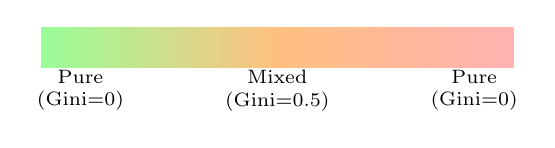
\begin{tikzpicture}
      % Spectrum bar pure -> mixed -> pure
      \shade[left color=green!40, right color=red!30, middle color=orange!50]
            (0,0) rectangle (6,0.5);
      \node[font=\scriptsize, align=center] at (0.5, -0.3) {Pure\\(Gini=0)};
      \node[font=\scriptsize, align=center] at (3.0, -0.3) {Mixed\\(Gini=0.5)};
      \node[font=\scriptsize, align=center] at (5.5, -0.3) {Pure\\(Gini=0)};
    \end{tikzpicture}
    \end{center}
    \vspace{0.15cm}
    We choose the split that \textit{maximises purity} of the resulting child nodes.
\end{frame}

\begin{frame}{Decision Trees: Key Points}
    \begin{columns}[T,onlytextwidth]
        \column{0.5\textwidth}
        \textbf{Strengths}
        \begin{itemize}
            \item Highly interpretable — can draw the tree.
            \item Handles mixed feature types.
            \item No feature scaling required.
        \end{itemize}
        \column{0.5\textwidth}
        \textbf{Limitations}
        \begin{itemize}
            \item Prone to overfitting (deep trees).
            \item Unstable — small data changes can flip the tree.
            \item Axis-aligned splits only.
        \end{itemize}
    \end{columns}
    \vspace{0.25cm}
    Extensions overcome limitations: \textbf{Random Forests} (many trees + voting), \textbf{Gradient Boosting}.

    \vspace{0.15cm}
    Real-world uses: medical triage, loan approval, customer churn diagnosis.
\end{frame}

% ======================================================
\section{k-Means Clustering}
% ======================================================

\begin{frame}{k-Means: The Idea}
    \textbf{Unsupervised.} Group $n$ data points into $k$ clusters such that points within a cluster are \textbf{as similar as possible}.

    \vspace{0.2cm}
    \begin{center}
    \begin{tikzpicture}
      % Three clusters
      \foreach \x/\y in {0.3/2.5, 0.5/2.0, 0.8/2.7, 0.6/2.2, 0.4/2.8}
        \fill[mDarkTeal!60] (\x*2,\y) circle (3pt);
      \foreach \x/\y in {2.0/0.4, 2.3/0.8, 2.6/0.3, 2.2/0.6, 2.5/1.0}
        \fill[orange!80!black] (\x*2,\y) circle (3pt);
      \foreach \x/\y in {3.5/2.0, 3.8/2.4, 4.0/1.8, 3.7/2.6, 4.2/2.2}
        \fill[green!60!black] (\x,\y) circle (3pt);
      % Centroids
      \fill[mDarkTeal, star, star points=5] (1.1, 2.45) circle (4pt);
      \fill[orange!60!black, star, star points=5] (4.5, 0.62) circle (4pt);
      \fill[green!40!black, star, star points=5] (3.84, 2.2) circle (4pt);
      \node[font=\scriptsize] at (4.0, -0.2) {$\bigstar$ = centroid};
    \end{tikzpicture}
    \end{center}
\end{frame}

\begin{frame}{k-Means: The Algorithm}
    \begin{center}
    \resizebox{0.86\textwidth}{!}{%
    \begin{tikzpicture}[node distance=0.65cm]
      \node[box] (init) {1. Randomly place\\$k$ centroids};
      \node[box, right=0.8cm of init] (assign) {2. Assign each point\\to nearest centroid};
      \node[box, right=0.8cm of assign] (update) {3. Move centroids\\to cluster mean};
      \node[greenbox, below=0.75cm of assign] (conv) {Converged?\\(centroids stable)};
  \node[greenbox, right=0.8cm of conv] (done) {Done};

      \draw[arrow] (init) -- (assign);
      \draw[arrow] (assign) -- (update);
      \draw[arrow] (update) -- (conv);
  \draw[arrow] (conv.east) -- node[above, font=\tiny]{Yes} (done.west);
  \draw[arrow, dashed, mDarkTeal!70] (conv.west) -- ++(-0.35,0) |- node[pos=0.2, left, font=\tiny]{No} (assign.south);
    \end{tikzpicture}
        }
    \end{center}
\end{frame}

\begin{frame}{k-Means: Step-by-Step Visualisation}
    \begin{columns}[T,onlytextwidth]
        \column{0.33\textwidth}
        \textbf{Step 1: Initialise}
        \begin{center}
        \begin{tikzpicture}[scale=0.7]
          \foreach \x/\y in {0.3/0.4, 0.6/0.8, 1.0/0.5, 2.0/1.8, 2.3/2.0, 1.8/2.2, 3.5/0.6, 3.8/0.3, 3.3/0.8}
            \fill[mDarkTeal!50] (\x,\y) circle (2.5pt);
          \fill[red!80]    (0.5, 1.5) circle (4pt);
          \fill[orange!80] (2.5, 0.5) circle (4pt);
          \fill[green!60!black]  (3.0, 2.0) circle (4pt);
        \end{tikzpicture}
        \end{center}

        \column{0.33\textwidth}
        \textbf{Step 2: Assign}
        \begin{center}
        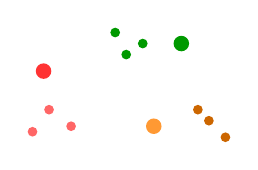
\begin{tikzpicture}[scale=0.7]
          \foreach \x/\y in {0.3/0.4, 0.6/0.8, 1.0/0.5}
            \fill[red!60] (\x,\y) circle (2.5pt);
          \foreach \x/\y in {2.0/1.8, 2.3/2.0, 1.8/2.2}
            \fill[green!60!black] (\x,\y) circle (2.5pt);
          \foreach \x/\y in {3.5/0.6, 3.8/0.3, 3.3/0.8}
            \fill[orange!80!black] (\x,\y) circle (2.5pt);
          \fill[red!80]    (0.5, 1.5) circle (4pt);
          \fill[orange!80] (2.5, 0.5) circle (4pt);
          \fill[green!60!black]  (3.0, 2.0) circle (4pt);
        \end{tikzpicture}
        \end{center}

        \column{0.33\textwidth}
        \textbf{Step 3: Update}
        \begin{center}
        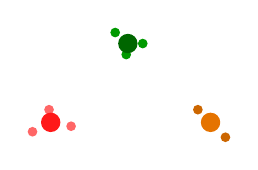
\begin{tikzpicture}[scale=0.7]
          \foreach \x/\y in {0.3/0.4, 0.6/0.8, 1.0/0.5}
            \fill[red!60] (\x,\y) circle (2.5pt);
          \foreach \x/\y in {2.0/1.8, 2.3/2.0, 1.8/2.2}
            \fill[green!60!black] (\x,\y) circle (2.5pt);
          \foreach \x/\y in {3.5/0.6, 3.8/0.3, 3.3/0.8}
            \fill[orange!80!black] (\x,\y) circle (2.5pt);
          % New centroids
          \fill[red!90]    (0.63, 0.57) circle (5pt);
          \fill[orange!90!black] (3.53, 0.57) circle (5pt);
          \fill[green!40!black]  (2.03, 2.0)  circle (5pt);
        \end{tikzpicture}
        \end{center}
    \end{columns}
\end{frame}

\begin{frame}{Choosing $k$: The Elbow Method}
    \begin{center}
    \begin{tikzpicture}
      \draw[-Stealth] (0,0) -- (5.5,0) node[right, font=\scriptsize]{$k$ (number of clusters)};
      \draw[-Stealth] (0,0) -- (0,3.0) node[above, font=\scriptsize]{Within-cluster sum of squares (WCSS)};

      \draw[mDarkTeal, thick] plot[smooth] coordinates
            {(0.5,2.8)(1,2.1)(2,1.1)(3,0.75)(4,0.62)(5,0.58)};

      % Elbow annotation
      \fill[orange!80!black] (2, 1.1) circle (3pt);
      \draw[dashed, orange!80!black] (2, 1.1) -- (2, 0)
            node[below, font=\scriptsize, orange!80!black]{$k=3$ (elbow)};
    \end{tikzpicture}
    \end{center}
    \vspace{0.1cm}
    At the elbow, adding more clusters gives \textit{diminishing returns} in compactness.
\end{frame}

\begin{frame}{k-Means: Key Points}
    \begin{columns}[T,onlytextwidth]
        \column{0.5\textwidth}
        \textbf{Strengths}
        \begin{itemize}
            \item Simple and fast.
            \item Scales to large datasets.
            \item Easy to interpret clusters.
        \end{itemize}
        \column{0.5\textwidth}
        \textbf{Limitations}
        \begin{itemize}
            \item Must choose $k$ in advance.
            \item Sensitive to initialisation and outliers.
            \item Assumes spherical, equally sized clusters.
        \end{itemize}
    \end{columns}
    \vspace{0.3cm}
    Real-world uses: customer segmentation, image compression, document grouping, geo-spatial analysis.
\end{frame}

% ======================================================
\section{Comparing the Algorithms}
% ======================================================

\begin{frame}{Algorithm Comparison at a Glance}
    \footnotesize
    \setlength{\tabcolsep}{3pt}
    \renewcommand{\arraystretch}{1.2}
    \begin{tabularx}{\textwidth}{>{\raggedright\arraybackslash}p{2.3cm} *{4}{>{\centering\arraybackslash}X}}
        \toprule
        \textbf{Aspect} & \textbf{Lin.\ Reg.} & \textbf{k-NN} & \textbf{Dec.\ Tree} & \textbf{k-Means} \\
        \midrule
        Type & Supervised & Supervised & Supervised & Unsupervised \\
        Task & Regression & Both & Both & Clustering \\
        Interpretable & Yes & Moderate & Yes & Moderate \\
        Training speed & Fast & Instant & Moderate & Moderate \\
        Prediction speed & Fast & Slow & Fast & — \\
        Handles non-linear & No & Yes & Yes & — \\
        \bottomrule
    \end{tabularx}
\end{frame}

% ======================================================
\section{Assessment and Wrap-Up}
% ======================================================

\begin{frame}{Assessment Q1 — What is Learning?}
    \textbf{Question:} Explain the difference between a hand-coded rule system and a machine learning model using a spam filter as your example.

    \vspace{0.2cm}
    \textbf{Expected points:}
    \begin{itemize}
        \item Rule system: engineer writes rules (``if subject contains `free money' → spam'').
        \item ML: algorithm infers rules from thousands of labelled emails.
        \item ML adapts when spammers change tactics; rules must be updated manually.
    \end{itemize}
\end{frame}

\begin{frame}{Assessment Q2 — Supervised vs Unsupervised}
    Classify each scenario (with justification):
    \begin{enumerate}
        \item Predicting whether a loan applicant will default.
        \item Grouping hospital patients by symptom similarity (no diagnosis yet).
        \item Estimating tomorrow's electricity demand from historical usage.
        \item Detecting unusual network traffic with no prior examples of attacks.
    \end{enumerate}
\end{frame}

\begin{frame}{Assessment Q3 — Overfitting}
    A model achieves 99\% accuracy on training data and 61\% on test data.

    \begin{itemize}
        \item What is this phenomenon called?
        \item What are two likely causes?
        \item Propose two concrete remedies.
    \end{itemize}
\end{frame}

\begin{frame}{Assessment Q4 — Algorithm Choice}
    For each task below, state which algorithm you would \textit{first try} and why:
    \begin{enumerate}
        \item Predicting the sale price of a house given its features.
        \item Classifying handwritten digits (0–9).
        \item Segmenting 10,000 retail customers into groups with no prior labels.
        \item Determining whether a tumour is malignant based on biopsy features.
    \end{enumerate}
\end{frame}

\begin{frame}{Assessment Q5 — Decision Trees \& Overfitting}
    \textbf{Scenario:} You train a decision tree and notice it perfectly classifies all training data but performs poorly on validation data.

    \vspace{0.2cm}
    \begin{itemize}
        \item Draw (or describe) what an over-grown decision tree looks like.
        \item What does \textit{pruning} mean and how does it help?
        \item How would using a \textbf{Random Forest} address this issue?
    \end{itemize}
\end{frame}

\begin{frame}{Key Takeaways}
    \begin{enumerate}
        \item \textbf{Learning} = improving performance on tasks through experience (data).
        \item \textbf{Supervised learning} uses labelled data; \textbf{unsupervised} finds hidden structure.
        \item Always split data into \textbf{train / validation / test} — never evaluate on training data.
        \item \textbf{Overfitting} memorises noise; \textbf{underfitting} misses the signal. Tune complexity.
        \item Four core algorithms:
        \begin{itemize}
            \item \textbf{Linear Regression} — predict continuous values with a line.
            \item \textbf{k-NN} — classify by neighbour majority vote.
            \item \textbf{Decision Trees} — hierarchical if-then rules.
            \item \textbf{k-Means} — find clusters by iterating assignments and centroids.
        \end{itemize}
    \end{enumerate}
\end{frame}

\begin{frame}[standout]
    Questions?
\end{frame}

\end{document}
